\section{RL basics}
Firstly, an environment where an agent can operate must be defined. The environment can be described as Markov decision process, where $S_t \in \mathcal{S}$ is a state from a set of possible states $\mathcal{S}$ in which environment is located in time $t$. An agent can usually observe the state of the environment and take action accordingly. An action is a probabilistic transition between states. Every action $A_t \in \mathcal{A}$ moves the environment from $S_t$ to $S_{t+1}$. The environment evaluates every action and returns appropriate reward $R_t$ (figure \ref{fig:rlconcept}). In RL set $\mathcal{A}$ is often called action space and set $\mathcal{S}$ observation space. The main goal of the agent is to find policy $\pi$ which maximizes expected return. Return $G_t$ is a sum of discounted future rewards \cite{sutton2012}.
\begin{equation}
G_t = \sum\limits_{k=0}^{\infty}\gamma^k R_{t+k}
\end{equation}
where $\gamma \in [0,1]$ is discount factor. RL methods define how experiences from interacting with the environment will change the policy.  The major issue is that maximizing immediate reward is often not an effective approach to maximize an expected sum of discounted rewards. This greedy policy can take the agent into a very disadvantageous state. Thus, the agent must take into account future states and rewards. This is done by value function $V_pi(S_t)$ which assesses how advantageous is being in state $S_t$ with policy $\pi$.
\begin{equation}
V_\pi(S_t) \doteq  \mathbf{E}_\pi[G_t | S_t].
\end{equation}
Optimal policy $\pi^*$ is then defined as
\begin{equation}
\pi^*(S_t) \doteq \max\limits_\pi V_\pi(S_t),
\end{equation}
for all $S_t \in \mathcal{S}$.
In the past agents used big tables to estimate the value function. That is possible in environments with small action and observation spaces but is very memory consuming for larger environments and even impossible for continuous action or observation space. Therefore, modern methods use neural networks as function estimators.
\begin{figure}[!h]
\centering
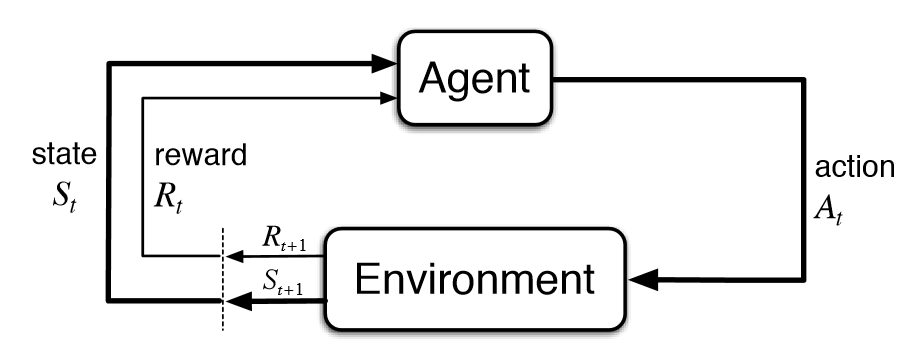
\includegraphics[scale=0.3]{fig/RL-concept.png}
\caption[RL concept]{RL concept. Source - \cite{sutton2012}.}
\label{fig:rlconcept}
\end{figure}
\pagebreak

\subsection{Temporal difference learning}
Temporal difference (TD) learning combines the ideas of Monte Carlo methods and dynamic programming. It can learn directly from experience obtained by interactions with an environment without any prior knowledge of the said environment. TD learning is done by following assignment in each timestamp \cite{sutton2012}
\begin{equation}
V(S_t) \gets V(S_t) + \lambda [R_{t} + \gamma V(S_{t+1}) - V(S_t)]
\end{equation}
where $\lambda \in \mathbb{R}^+$ is step size.

\subsection{Q-learning}
Q-learning is a type of TD learning developed by Watkins \cite{watkins1992}. The state value $V$ from the previous subsection is replaced by $Q$ value, which refers to a quality of action in a particular state instead of the quality of the state itself. When we rewrite TD learning (4) to Q-learning we get:
\begin{equation}
Q(S_t, A_t) \gets Q(S_t, A_t) + \lambda [R_{t} + \gamma \underset{A_{t+1}}{\max} Q(S_{t+1}, A_{t+1}) - Q(S_t, A_t)].
\end{equation}
Our policy here is to take action with maximal $Q$ value. That is called greedy policy. An obvious drawback of greedy policy is that it does not allow to explore the whole environment properly because an action with the highest $Q$ value is always chosen. A solution to this problem is sometimes to take random action to explore the environment. This policy is often referred to as $\epsilon$-greedy policy.

\begin{algorithm}
\caption{$\epsilon$-greedy policy in pseudocode}
\begin{algorithmic}[1]
\Procedure{ChooseAction}{}
\State $\epsilon \gets \epsilon \cdot \epsilon_d$
\If {$\epsilon >$ random $\in (0,1)$}
\State action $\gets$ random $\in \mathcal{A}$
\Else 
\State action $\gets$ $\underset{A_t}{\max} Q(S_t, A_t)$
\EndIf
\State \Return action
\EndProcedure
\end{algorithmic}
\end{algorithm}

It is common to set $\epsilon = 1$ at the beginning of the training and decay rate $\epsilon_d$ close to one. The general idea behind this policy assumes that it is needed to explore an environment first and then exploit agents experience.

\clearpage

\subsection{Prioritized experience replay}
Experience replay is biologically inspired mechanism introduced by Schaul et al. \cite{schaul2015} which stores all experiences (specifically: $S_t$, $A_t$, $R_{t}$, $S_{t+1}$) into a buffer and assigns priority to every experience. The main idea is that experiences with high TD should have higher priority. It is thus necessary to calculate priority $p$ from TD error:
\begin{equation}
p = (|\delta_t | + \eta)^\rho
\end{equation}
where $\rho$ indicates how much we prefer experiences with higher priority and $\eta \ll 1$ is a constant which helps to avoid priorities very close to zero. Considering a greedy selection would abandon experiences with low priority, a better approach is to choose experience $i \in \mathcal{I}$ with probability:
\begin{equation}
P(i) = \frac{p_i}{\sum\limits_{j \in \mathcal{I}} p_j},
\end{equation}
where $\mathcal{I}$ is set of all experiences in the buffer. It is possible now to sample a batch of experiences for training using this probability. It removes correlation in the observation sequence and improves sample efficiency of DQN. It is feasible to store all experiences in a buffer sorted by priority, but a more efficient implementation is a sum tree. That is a binary tree, where the value of each root is equal to the sum of its children values (see figure \ref{fig:sumtree}).
\begin{algorithm}
\caption{Retrieve node from sum tree in pseudocode}
\begin{algorithmic}[1]
\Procedure{GetChild(parent, value)}{}
\If {parent.left is None} \Return parent \EndIf
\If {value $\leq$ parent.left.value} 
\State \Return GetChild(parent.left, value)
\Else 
\State \Return GetChild(parent.right, value - parent.left.value)
\EndIf
\EndProcedure
\end{algorithmic}
\end{algorithm}
\begin{figure}[H]
\centering
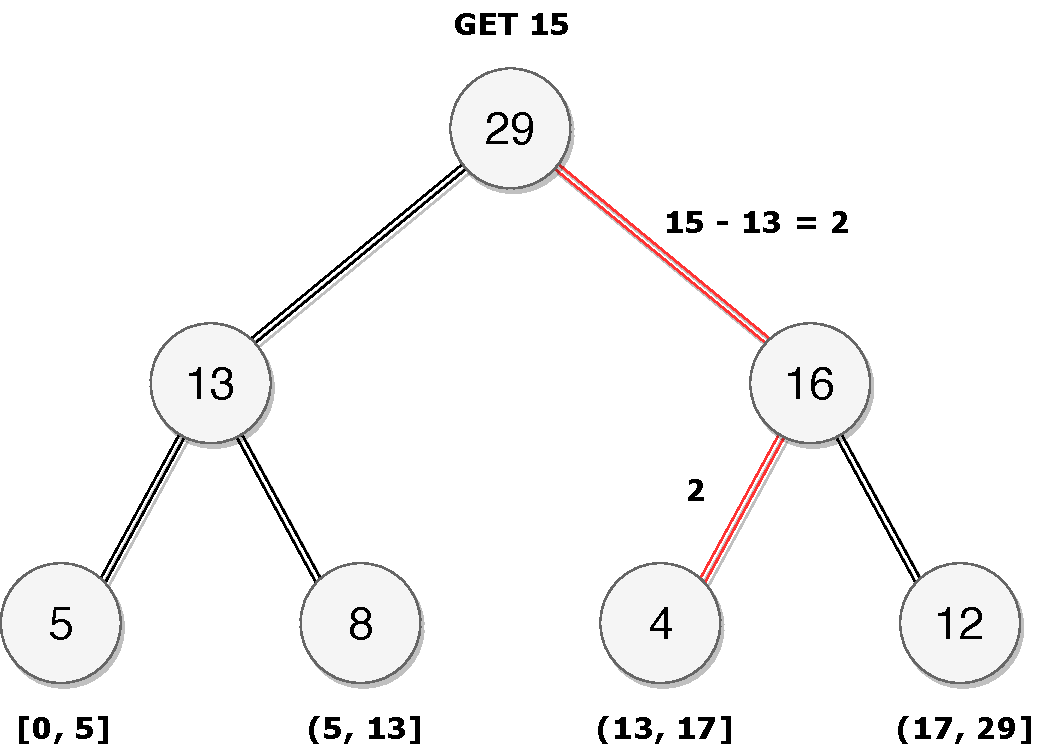
\includegraphics[scale=0.5]{fig/sumtree.pdf}
\caption[Sum tree]{Simple example of sum tree.}
\label{fig:sumtree}
\end{figure}
\clearpage
\section{Deep neural networks in RL}
As was stated in the previous chapter, tabular methods are very inefficient in large environments. In these instances, it is possible to use deep neural networks which can replace tables. Deep Q networks (DQN) proposed by Googles Deepmind \cite{mnih2015} outperformed all previous RL algorithms in playing Atari games. With neural networks also grew the popularity of policy gradient methods where function estimator outputs an action instead of Q values. Note that the most of these methods are general and not necessarily tied to neural networks.

\subsection{Deep Q network}
The neural network takes current state as input and outputs Q value for each possible action. The network is trained using gradients of Q-value in the current state with respect to trainable weights $\theta$ of our neural network.
\begin{align} \label{eq:qlearn}
\delta_t &= R_{t} + \gamma \underset{A_{t+1}}{\max}Q^\theta(S_{t+1}, A_{t+1}) - Q^\theta(S_t, A_t)\\
\theta_{t+1} &= \theta_t + \lambda \delta_t \nabla_\theta Q^\theta (S_t, A_t).
\end{align}
Gradients are updated in proportion to TD $\delta_t$. Unfortunately, this simple DQN agent suffers from a lack of sample efficiency and does not converge well. There are many techniques which can help DQNs to achieve satisfying results.

\subsection{Target network}
Target network is a technique which improves convergence of DQN learning \cite{mnih2015}. It uses two neural nets instead of one. The first is trained online network on a batch of data and the second target network is used for predictions during training. After the completion of training on a batch of data, the target network is updated.
\begin{equation}
\theta^- = \tau \theta + (1-\tau)\theta^-,
\end{equation}
where $\theta^-$ is set of trainable weights of the target network, $\theta$ indicates online network weights and $\tau \ll 1$ is constant.
TD $\delta$ is now calculated using target network:
\begin{equation}
\delta_t = R_{t} + \gamma \underset{A_{t+1}}{max}Q^{\theta^-}(S_{t+1}, A_{t+1}) - Q^\theta(S_t, A_t). 
\end{equation}
Target network stabilizes training since predicting network does not change after each training step.

\subsection{Double Q-learning}
Classic Q-learning algorithm tends to overestimate actions under certain conditions. Hasselt et al. propose the idea of Double Q-learning which decompose the max operation into action selection and action evaluation \cite{hasselt2015}. TD is then computed by the following equation.
\begin{equation}
\delta = R_{t} + \gamma Q^{\theta^-}(S_{t+1}, \underset{A_{t+1}}{\text{argmax}}Q^\theta(S_{t+1}, A_{t+1})) - Q^\theta (S_t, A_t).
\end{equation}
Double DQN outperforms DQN in terms of value accuracy and in terms of policy quality.

\clearpage
\section{Policy gradient}
By this section, the goal of the neural network was predicting values by which we determined the policy. In policy gradient method neural network approximates the policy itself. 
\begin{equation}
\theta_{t+1} = \theta_t + \lambda \widehat{\nabla J(\theta_t)}
\end{equation}
where $J$ is performance measure with respect to our neural network parameters and $\widehat{\nabla J(\theta_t)}$ is stochastic estimate which approximates gradient of the performance measure. In other words, this method is basically doing stochastic gradient ascent of $J$ with respect to $\theta$ \cite{sutton1999}. Policy gradient methods are outperforming DQNs, especially in continuous action spaces, because their output is directly continuous action instead of Q-value for every possible action.

\subsection{Actor-Critic}
Thanks to predicting action directly, we gain the possibility to predict in continuous action space, but the Q-value which assessed the quality of action in a certain state has been lost. That is why the Actor-Critic framework was created. It uses two separate neural networks - actor which predicts action and critic which assesses action advantage. Concept is visualised in the figure \ref{fig:actorcritic}.
\begin{figure}[H]
\centering
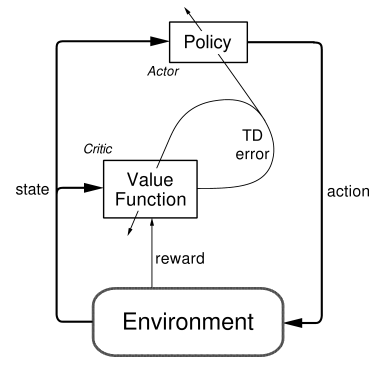
\includegraphics[scale=0.55]{fig/actor-critic.png}
\caption[Actor-Critic framework]{Actor-Critic framework. Source - \cite{sutton2012}.}
\label{fig:actorcritic}
\end{figure}
\clearpage

Consider critic using Q-values for the update. $\theta$ and $\omega$ denote trainable weights of actor and critic, respectively. Critic update is similar to DQN:
\begin{align}
\delta_t &= r_t + \gamma Q^\omega(S_{t+1}, \mu ^\theta (S_{t+1})) - Q^\omega(S_t, A_t)\\
\omega_{t+1} &= \omega_t + \lambda \delta_t \nabla_\omega Q^\omega(S_t, A_t).
\end{align}
Note that instead of $A_{t+1}$ is now used function $\mu^\theta(S)$, which is an action estimate by actor neural network. Actor update rule is not so straightforward. 
\begin{equation}
\theta_{t+1} = \theta_t + \lambda\nabla_\theta \mu^\theta(S_t)\nabla_a Q^\omega (S_t, A_t)|_{a = \mu^\theta(S_t)}.
\end{equation}
This equation uses chain rule for derivatives to obtain the gradient of Q-values with respect to trainable weights $\theta$. Namely:
\begin{equation}
\frac{\partial Q^\omega(S_t, A_t)}{\partial \theta} = \frac{\partial Q^\omega(S_t, A_t)}{\partial A_t} \frac{\partial A_t}{\partial \theta}.
\end{equation}
Actor neural network is updated by gradients which change action output to maximize Q-value of the critic \cite{silver2014}.
There are other approaches, which doesn't use Q-value as critic assessment, but they rather use so-called advantage \cite{schulman2017}. These methods are beyond the scope of this thesis. 

\subsection{Stochastic Actor-Critic}
A stochastic Actor-Critic method is frequently used approach. In this method actor outputs parameters of distribution and action itself is sampled within the parameterized distribution. It is standard to use normal distribution and predict the mean and variance of action. The biggest advantage of the normal distribution is that it can be adjusted to use of backpropagation \cite{hess2015}. Another benefit of the stochastic actor is that it does not need any other techniques for action space exploration.

\subsubsection{Beta distribution}
On the other hand, obvious drawback of the normal distribution is that there is always some small probability of sampling an outlier. There is also an issue for bounded action space. When mean value of the normal distribution is close to the boundary, an agent can experience not negligible bias. A solution for both problems is to use beta distribution as a stochastic policy \cite{chou17}. The beta distribution is defined by the following function:
\begin{equation}
f(x;\alpha, \beta) = \frac{\Gamma(\alpha + \beta)}{\Gamma(\alpha)\Gamma(\beta)}x^{\alpha-1}(1-x)^{\beta-1},
\end{equation}
where $\alpha,\beta \in R^+_0$ are distribution parameters and $x \in [0, 1]$. $\Gamma$ is Euler's gamma function, which extends factorial into the set of real numbers. Beta distribution is shown in the figure \ref{fig:beta}.

\begin{figure}[H]
\centering
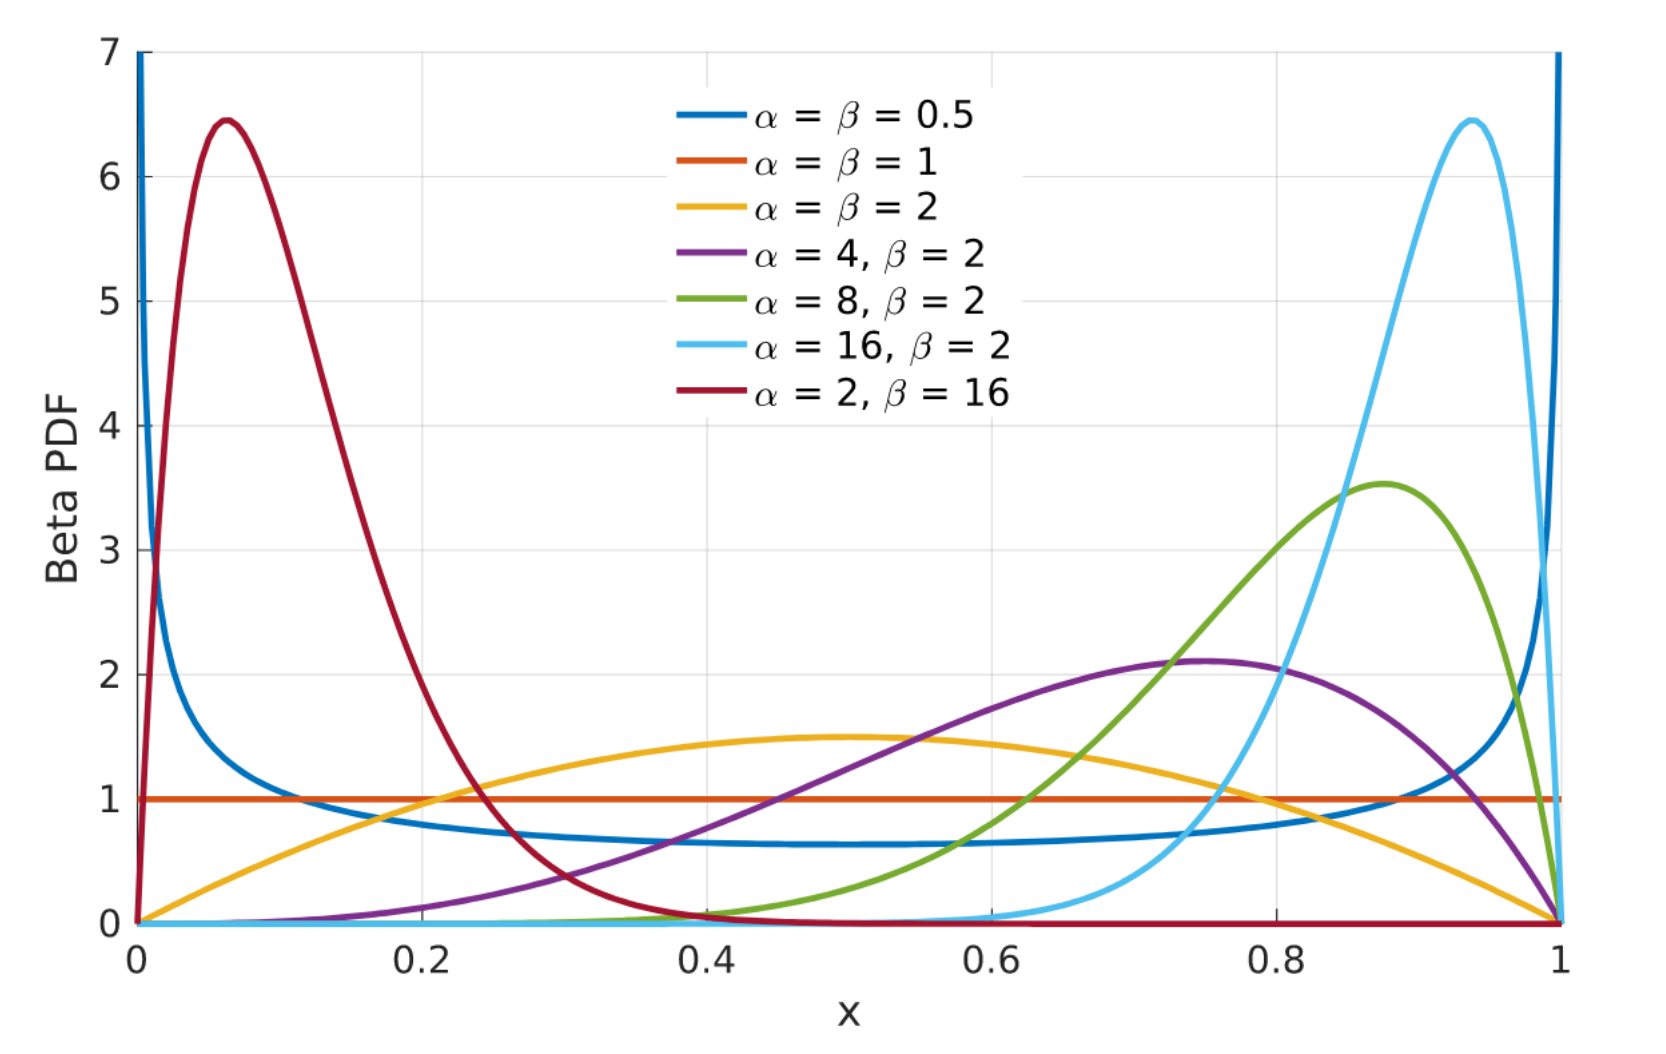
\includegraphics[scale=0.2]{fig/beta.png}
\caption[Probability density of beta distribution]{Probability density of beta distribution. Source - \cite{chou17}.}
\label{fig:beta}
\end{figure}

For reinforcement learning is suitable only $\alpha, \beta \geq 1$. That makes beta distribution concave and unimodal. It can be ensured by using softplus activation and adding one at the end of actor-network.

\subsection{Deterministic policy gradients}
Deep deterministic policy gradient (DDPG) is one of the methods for exploiting the Actor-Critic framework. Whereas stochastic actor predicts distribution parameters and samples an action DDPG outputs the action directly. Silver \cite{silver2014} has shown that deterministic policy can outperform its stochastic counterparts. A disadvantage of this approach is that it needs an additional policy to ensure action space exploration. Exploration methods are discussed in subsection \ref{sec:exploration}.

\subsection{Wolpetinger policy}
Actor-Critic methods and DDPG work well in continuous action spaces, but there are many use cases with large discrete action spaces, such as recommender systems or lidar planning. Wolpetinger policy is approach how to utilize continuous methods in discrete action space \cite{dulac2015}. The whole policy is illustrated in figure \ref{fig:wolpetinger}. An actor doesn't predict action directly, but it predicts so-called proto-action $\tilde{A_t}$.
\begin{equation}
\tilde{A_t} = \mu^\theta(S_t).
\end{equation}
Proto action mostly isn't valid action $\tilde{A_t} \notin \mathcal{A}$. Thus it is necessary to find the valid action corresponding to the proto action. That is done by computing Euclidean distance to every possible action.
\begin{equation} \label{eq:knn}
\mathcal{A}_{knn} = \overset{K}{\underset{a \in \mathcal{A}}{{\text{argmin}}}} | a - \tilde{A_t} |_2 .
\end{equation}
Usually, policy chooses $K$ closest actions to the proto action. $\mathcal{A}_{knn}$ is the set of closest action to the proto action. The whole set is then assessed by critic and action with highest Q-value is finally picked.
\begin{equation}
A_t = \underset{a \in \mathcal{A}_{knn}}{\text{argmax}} Q^\omega(S_t, a)
\end{equation}
\begin{figure}[!h]
\centering
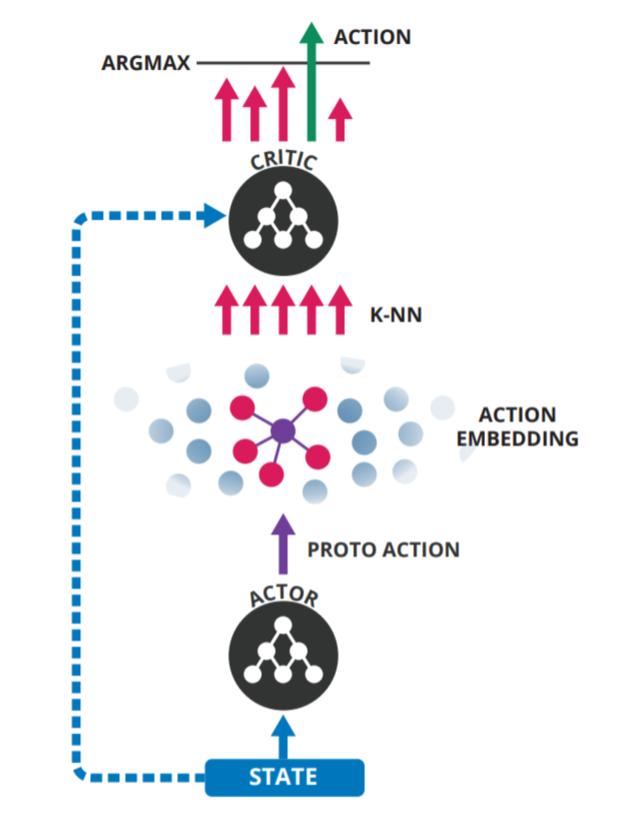
\includegraphics[scale=0.35]{fig/wolpetinger-policy.png}
\caption[Wolpetinger policy illustration] {Wolpetinger policy can be described in 3 steps. \textbf{1)} Actor outputs an action \textbf{2)} The $K$ nearest valid actions are found \textbf{3)} Choose the action which is assessed as the best by the critic. Source - \cite{dulac2015}.}
\label{fig:wolpetinger}
\end{figure}

\subsection{Parameter and action space noise}
\label{sec:exploration}
In large action, space is crucial to emphasize agents exploration. Bad exploration can cause that agent converges prematurely and ends up in a local optimum. DDPG commonly uses stochastic policy to modify actors actions slightly.
\begin{equation} \label{eq:exploration}
\hat{A_t} = \mu^\theta(S_t) + \mathcal{N}(0, \sigma^2)
\end{equation}
where $\mathcal{N}$ is the normal distribution with mean value equal to zero and variance, which is reducing during the training and $\hat{A_t}$ is perturbed action. Action space noise helps agent to explore the environment. \par Another approach is to apply noise directly to actors weights. It can sometimes lead to more consistent exploration and richer behaviors \cite{plappert2017}.
\begin{equation}
\hat{\theta} = \theta + \mathcal{N}(0, \sigma^2)
\end{equation}
where $\hat{\theta}$ is a so-called perturbed actor, which is interacting with an environment. The major issue of parameter space noise is that it is much harder to tune. When we use action space noise, it is easy to estimate its impact on actions (differences between both approaches can be seen in the figure \ref{fig:exploration}). Because of an unpredictable influence of parameter space noise is necessary to use adaptive noise scaling.
\begin{align}
d &= |\hat{A_t} - \mu^\theta(S_t)|_2  \\
\sigma_{t+1} &= 
     \begin{cases}
       \kappa \sigma_t & \text{if } d \leq T \\
       \frac{1}{\kappa}\sigma_t & \text{otherwise}
     \end{cases}
\end{align}
where $\kappa$ is scaling factor slightly bigger than one and $T$ is the threshold value, which has to be tuned to a specific environment.
\par When is necessary to explore action space near to some specific action or include momentum of an environment, it is possible to use Ornstein-Uhlenbeck random process \citep{lilicrap2015}. 
\begin{equation}
\hat{A_t} = \mu^\theta(S_t)  + \nu (\rho - \mu^\theta(S_t)) + \phi \mathcal{N}(0, 1),
\end{equation}
where $\nu, \phi \in [0, 1]$ are constants of the random process and $\nu$ is mean value around which we want to explore the action space. When $\nu = 0$ it is basic exploration as in expression \eqref{eq:exploration}.

\begin{figure}[H]
\centering
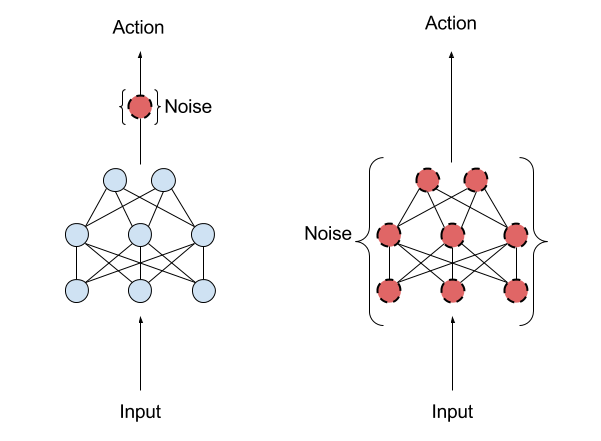
\includegraphics[scale=0.5]{fig/perturbations.png}
\caption[Exploration noise types]{Left - action space noise, Right - parameter space noise. Source - \cite{plappert2017}.}
\label{fig:exploration}
\end{figure}